% ==============================================================================
%
% "Ideas for Citizen Science in Astronomy"
%
% Marshall, Fletcher, & Lintott, ARAA (2015)
%
% ==============================================================================

\documentclass{ar2e}

\usepackage{ulem}
\usepackage{ARAstroBib}
\usepackage{amssymb,amsbsy,psfig}
\usepackage{xspace}
\usepackage[usenames]{color}
\usepackage{graphicx}

% JOURNALS
\def\apj{ApJ}                                         
\def\apjs{ApJS}
\def\apjl{ApJL}
\def\aap{A{\&}A}
\def\aaps{A{\&}AS}
\def\mnras{MNRAS}
\def\aj{AJ}
\def\araa{ARAA}
\def\pasp{PASP}
\def\nat{Nature}
\def\prd{Phys.\ Rev.\ D}

% MISC
\def\eg{{\it e.g.}\xspace}
\def\ie{{\it i.e.}\xspace}
\def\cf{{\it c.f.}\xspace}
\def\etal{et~al.\xspace}

% CROSS-REFERENCES
\def\Sref#1{Section~\ref{#1}\xspace}
\def\Fref#1{Figure~\ref{#1}\xspace}
\def\Tref#1{Table~\ref{#1}\xspace}
\def\Eref#1{Equation~\ref{#1}\xspace}
\def\Eqref#1{Eq.~(\ref{#1})\xspace}

% COMMENTING
\newcommand{\phil}[1]{\textcolor{blue}{\bf PJM: #1}}
\newcommand{\chris}[1]{\textcolor{blue}{\bf CJL: #1}}
\newcommand{\leigh}[1]{\textcolor{blue}{\bf LDF: #1}}
\newcommand{\todo}[2]{{\bf \it TODO: #1: #2}}
\newcommand{\query}[2]{{\it \textcolor{red}{Q: #1: #2}}}
\newcommand{\answer}[2]{{\it \textcolor{blue}{A: #1: #2}}}


% ==============================================================================

\begin{document}

% ------------------------------------------------------------------------------

\jname{Annu.\ Rev.\ Astron.\ Astrophys.}
\jyear{2014}
\jvol{}
\ARinfo{}

\title{Ideas for Citizen Science in Astronomy}

\author{Phil Marshall,$^{1,2}$
Leigh Fletcher,$^{2}$ and
Chris Lintott$^{2}$
\affiliation{%
\small
$^1$ Kavli Institute for Particle Astrophysics and Cosmology, P.O.~Box~20450, \newline
MS~29, Stanford, CA 94309, USA. \newline
$^2$ Department of Physics, Denys Wilkinson Building, University of Oxford, \newline
Keble Road, Oxford, OX1 3RH, UK.}}

\markboth{Marshall, Lintott \& Fletcher}{Citizen Astronomy}

% ------------------------------------------------------------------------------

% \begin{keywords}
% Go here...
% \end{keywords}

\begin{abstract} 

We review the relatively new, internet-enabled, and rapidly evolving field of
citizen science, focusing on projects in astronomy and solar system science but
sampling beyond those fields. In doing so, we look for  ideas from which
astronomy  could benefit in the future. We consider contributions to science in
the form of observations, data processing, data modeling and the design of new
scientific inquiries, and from this experience derive some commonalities between
the most successful projects, and use them to suggest some guidelines for future
projects. The limits of citizen science are not yet well understood, but we make
some speculations for citizen astronomy in particular.

\todo{Phil}{Work conclusions into abstract}

\end{abstract}

\maketitle

% ==============================================================================

\section{Introduction (2 pages)}
\label{sec:intro}

The term ``citizen science'' refers to the activities of people who are not paid
to carry out scientific research, but who make intellectual contributions to
scientific research nonetheless.\footnote{In this review we differentiate
between the data analysis that citizens carry out themselves, and  distributed
``grid'' computing farmed out to computers owned by citizens, and omit the
latter since it does not fit our definition of citizen science as involving
intellectual  contributions from citizens.} They come from all walks of life,
and their contributions are diverse, both in type and research area. This review
is about the science projects they have participated in to date, the tasks they
have performed, and how astronomy has benefited -- and could benefit further --
from their efforts.

Citizen involvement in science pre-dates the profession itself, and there is a
long and honourable tradition of amateur observers making important discoveries
and significant sustained contributions. \question{Chris}{Does this statement
need justifying with some examples and/or citations?} However, the advent of the
world wide web has changed the face of professional and amateur collaboration,
providing new opportunities and accelerating the sharing of information. People
are now connected to each other on a scale that has never happened before.
Professional scientists can interact with citizens via a range of web-based
media, including on purpose-built citizen science websites which increase the
potential for shared data analysis and exploration, as well as for data
collection. Meanwhile, communities of citizens have sprung into existence as
like-minded people have been able to find and talk to each other in a way that
is almost independent of their geographical location. The result has been an
exponential increase in citizen involvement in science. The field is evolving
very quickly, with more and more professional scientists becoming aware of the
possibilities offered by collaborating with, for example, specialists operating
outside the usual parameters of professional astronomical observation, or tens
of thousands of people eager to perform microtasks in their spare time.  

Our aim in this work is to review the scientific literature as it stands for
ideas implemented in citizen science projects, primarily in astronomy but
occasionally in other fields, and then produce a summary of successful project
characteristics for future research groups to learn from.  As our title states,
this is a review of ideas for astronomy. We will look forward as well as back,
and try to answer the questions: How can the full potential of citizen science
be realised in astronomy? What are the particular niches that citizen science
can fill, in our field? How might it contribute to the solutions of the Big Data
problem in astronomy?


This review is organised as follows. We survey the contributions to science that
citizens have made to date, organized according to the stage of the scientific
enquiry that those contributions fell into. Astronomy research typically starts
with observations: so do we, in \Sref{sec:obs}. We then proceed to consider 
visual classification, data modeling and finally citizen-led enquiry in 
Sections~\ref{sec:class}--\ref{sec:explore}. With this overview in place, we
review in \Sref{sec:crowd} the literature on, and the collected experience of,
the population of citizens who have taken part, or are currently taking part, in
scientific research. We then turn to the future, and speculate on how citizens
might contribute to astronomy there (\Sref{sec:future}); in  \Sref{sec:limits}
we consider possible limits to citizen science, including challenges associated
with data rates and volumes, data complexity, the difficulties of large-scale
collaboration, and the barriers to accessibility. Finally, we make some
concluding remarks in \Sref{sec:conclusions}, and suggest some guidelines for
the implementation of future citizen science projects in astronomy.


% ------------------------------------------------------------------------------

\section{Data Acquisition: Citizen Observing (5 pages)}
\label{sec:obs}

There is currently an active community of well-equipped amateur observers making
astronomical observations of great utility. There are also many other citizens
observing the night sky with less sophisticated equipment -- and as we shall
see, there are even citizens making  astronomical observations almost
inadvertently. What astronomical data are the citizenry taking, and what is it
being used for?


% - - - - - - - - - - - - - - - - - - - - - - - - - - - - - - - - - - - - - - - 

\subsection{Active Observing (3 pages)}
\label{sec:obs:active}

\todo{Phil}{Shorten solar system parts of active observations.}

\todo{Chris,Phil}{Write about galactic and extragalactic observations.}

The steady improvements and increasing affordability of digital technology, in
addition to the ease of data sharing and communications, have considerably
expanded the realm of amateur astronomy in the past two decades.  
% Observers have always been passionate about their pastime, from painstakingly
% recorded hand drawings of the planets and their positions in the night sky, to
% hours devoted to the monitoring and tracking of astronomical events.  There is a
% long and proud history of contributions from ``amateurs'' to the field, driven
% by a desire to share the results of their hobby with others, but it has only
% been in the past few decades that mechanisms have been in place that enable the
% sharing of large amounts of data between amateurs and professionals, enticing
% passionate observers to shape their observations to address scientific
% questions.  
In this section, we review some of the citizen contributions to active
observations of the night sky.  Passive contributions, via data mining and
web-based studies, will be described in \Sref{sec:obs:passive} below.

How is active citizen observing beneficial to astronomy research? 
\todo{All}{We give three benefits to the pro community of amateur observing:
time availability, flexibility and context. We should discuss this to make sure
we have a complete picture.} 

The first key advantage is time availability: professional observatories are
always over-subscribed, with resources ending up being concentrated on one area
of sky, or on a few astronomical questions.  Such observations are rarely tuned
to the optimum timescales for other scientific enquiries: for example,
determinations of meteor frequencies on short timescales (minutes), or slow
evolution of giant planets on longer timescales (years and decades).  In
contrast, amateur observations can be frequent, repetitive, and long standing,
and are naturally well sampled across the globe during an exciting event of
interest. 

The second, related, advantage is that of flexibility: whenever a new phenomenon
is discovered (e.g., a new comet, or anything changing the appearance of the
familiar planetary discs), observers will be keen to catch a glimpse
irrespective of the scientific value of their observations.  This reaction can
be near instantaneous, compared to the need to allocate telescope resources
among the professional community.  

The third benefit is contextual.  Professional observations often are taken in a
very different wavelength range, focus on a narrower spatial region, or employ
spectroscopic techniques that don't yield images. In some situations,
near-simultaneous wide field optical imaging by citizen scientists can provide
useful additional constraints on the process of interest.

The example case studies below serve to illustrate this synergy between amateur
and professional observations, and also to highlight instances of
professional-amateur (``Pro-Am'') collaboration. While the solar system provides
some of the most amenable targets for amateur observation, ``deep sky''
observations by the non-professional community provide important further insight
into the capabilities and potential of citizen astronomers.

% Instrumentation built and used by citizen scientists have increased in
% sophistication: complex personal observatories with large-aperture motorised
% telescope, multiple filters, and high precision low-light cameras have all
% become {\it de rigeur}.  Increasingly sophisticated software is also now
% available to aid in the reduction and quantitative analysis of amateur imaging,
% as described in \Sref{} below.  Vibrationally-damped mounts, advanced CCD and
% CMOS detectors, and a GOTO system to mechanically move to a set of celestial
% coordinates and track that location all serve to optimise the amount of time the
% observer actually gets to spend looking at the sky, and paves the way for fully
% robotic observatories.  The reader is referred to \citet{13mousis} for a
% thorough review of instrumentation currently in use for solar system studies.


% Comparisons with the visible albedo provided by citizen
% scientists can play an extremely useful role in planetary missions,
% both for context and for observation planning.  
% 
% Active observation by enthusiastic citizens contributing directly to scientific
% progress, combined with new excellent communication channels  and the digital
% technology that allows astrophotographers to shine, is beginning to plug this
% observational gap.
% 
% As a result of these benefits, a few professional solar system scientists are
% very closely linked with the amateur community, organising publications and
% assisting in observation planning to maximise science return.  
% 
% New planetary missions frequently involve scientists to serve as an interface
% with the amateur community (this is particularly true of the 2016-17 Juno
% mission to Jupiter).  In return, amateurs trigger alerts through online forums
% or emails to professional networks, announcing a tentative new discovery to the
% world for scrutiny and follow-up. 
%  
% The benefits of strong professional-amateur (``Pro-Am'')
% collaboration will be repeated in the following examples where active
% observations have contributed directly to our understanding of our place in the
% universe.  We do not intend a complete review of all examples of Pro-Am
% collaboration, but give a few representative examples.  For a detailed review of
% the methodology employed by amateur observers in solar system science, the
% reader is referred to \citet{13mousis}.  
% 
% Within our solar system, active observations fall into two interconnected
% categories:  Discovery and Monitoring, where each will almost certainly lead to
% the other.
% 
% \todo{Phil and Chris}{The previous two paragraphs had a distinctly solar system
% flavour. We should discuss them and edit them to make sure this section is
% general.}


% % -  -  -  -  -  -  -  -  -  -  -  -  -  -  -  -  -  -  -  -  -  -  -  -  -  - 
% 
% \subsubsection{Solar System Observations}


\CaseStudy{Discovering and Charecterizing Asteroids and Comets.}
Although survey telescopes provide the vast majority of modern solar system
discoveries, citizen astronomers occupy some interesting observational niches,
making discoveries in the places professional observatories can't reach. Targets
include near-earth asteroids (NEAs, with orbits intersecting those of the
terrestrial planets), main belt asteroids between Mars and Jupiter, and comets
making their journey towards the Sun from the outer solar system. A protocol for
citizen discovery has been established: the position of any new object is
compared to existing catalogues, and if no existing details are found then the
new discovery and its ephemerides can be reported to the IAU Minor Planet
Centre\footnote{http://www.minorplanetcenter.net}.   If observations are
repeated for at least two nights by one or several observers, then a new
denomination is provisionally assigned to the discovery.   An electronic
circular then reports the discovery to the wider world.

Small solar system objects moving against the fixed-star background can be
detected in a set of CCD frames either by eye or by automated software. The
extreme familiarity of citizen astronomers with a particular region, planet or
nebula, allowing them to immediately identify peculiarities or new features (a
good example of this is the study of meteorological activity on giant planets
\citep{95rogers}).   [For example?] the recent close flyby of asteroid 2012 DA14
on February 15th 2013 was initially reported by a team of amateur observers
affiliated with the La Sagra Sky Survey at the Astronomical Observatory of
Mallorca. \todo{Leigh}{add reference for 2012 DA14. How did they spot it? By eye
or with automated detection software? If all the amateur detection is being done
by eye we need to note that -- and in any case this paragraph will need
finishing.} 

Some amateur observers have been involved in new cometary discoveries, including
David Levy, part of the team that discovered Shoemaker-Levy 9 before its
spectacular impact with Jupiter.  \todo{Leigh}{add reference for
Shoemaker-Levy?} As with asteroids, the majority of new comet discoveries are
made by automated surveys, but a small and stable number of discoveries come
from amateurs with small telescopes, typically in regions poorly covered by
survey telescopes (e.g., regions close to the Sun).   C/2011 W3 Lovejoy, a
Kreutz sungrazer comet, is one such example.  C/2012 S1 ISON was spotted by A.
Novichonok and V. Gerke in images from the International Scientific Optical
Network. \todo{Leigh}{add reference for C/2012 S1 ISON?} 

Amateurs are also contributing to the search for a sub-category of objects
with a detectable cometary coma within the asteroid belt.  Recent discoveries
of these Main Belt Comets, which appear to be asteroids that are actively
venting their volatiles at perihelion, are beginning to blur the distinction
between asteroids and comets.  The T3 project, a collaboration between the
University of Rome and several amateur observers, began in 2005 with the
detection of a coma around asteroid 2005 SB216 \citep{05buzzi}, and has gone
on to detect at least eight main belt comets \citep{13mousis}. Comae may be
detected as an extended FWHM of the asteroid compared to the background stars,
or visually distinctive cometary comae.\footnote{Recent discoveries of cometary
activity can be found here: \texttt{http://schiaparelli204.wordpress.com/}}

Citizen observations allow detailed characterisation of physical and orbital
characteristics of these newly discovered solar system bodies, and amateur-led
contributions are published
online.\footnote{http://www.minorplanet.info/mpbdownloads.html}  There is a need
to continuously track Near Earth Asteroids as gravitational effects can
significantly alter orbital trajectories over time, and this astrometry for both
asteroids and comets can be provided to the Minor Planet Centre for collation
and use in computing orbital trajectories.  

Amateur monitoring of a comet's coma, dust and plasma tails and their
photometric parameters can reveal dynamic structures and determine the locations
of active venting regions.  Photometric monitoring of comets over time of the
magnitude and tail characteristics provides insights into the levels of activity
as the comet moves along its trajectory, and can also reveal outbursts and other
events associated with the outgassing.  Photometric monitoring of an asteroid as
it rotates provides information on the physical parameters, such as the shape,
rotation rate and orientation.  Observations of mutual encounters can also yield
information on the density, and hence the composition of the asteroids.
\todo{Leigh}{Add refs for monitoring comets, asteroids etc.}


\CaseStudy{Monitoring the Planets.} 

\todo{Leigh}{Please read this case study carefully, and please rearrange so that
it makes sense: I worry that I have not merged the software and observing parts
well. Could it be split into two or three, on order to better focus on the
various techniques? Or, could it be compressed into a shorter version?}

Jupiter's size, brightness and colourful cloud contrasts make it an ideal target
for citizen monitoring.  Winds, waves, storms and plumes shape the day-to-day
appearance, with cloud structures being blown east and west by powerful zonal
jets.  The jet velocities, and the dispersion of cloud material, reveals
processes at work beneath the visible ammonia ice clouds, and serve as a probe
of the fluid dynamics at work.  Tracking the motion of features requires
correlation of images obtained night after night; with filters sounding in and
out of strong jovian methane absorption features providing a three dimensional
view of the planet's cloud decks.  Monitoring studies are also underway for
Saturn, Uranus and Neptune, with increasing levels of difficulty. 

The global distribution of giant planet observers permits global monitoring of
Jupiter and Saturn as they rotate over 10 hours. Citizens upload raw filtered
images and colour composites, organised by date and time, to online servers,
such as the Planetary Virtual Observatory and Laboratory
(PVOL\footnote{\texttt{http://www.pvol.ehu.es/pvol}}) maintained for the
International Outer Planets Watch \citep[IOPW][]{10hueso}.  Those images can be
used by amateurs and professionals alike to quantitatively study the zoology of
activity; from measuring wind speeds \citep{08sanchez}; investigating the
strength and changes to the large vortices \citep[e.g., the 2006 reddening of
Oval BA,][]{06simon-miller}; to determining the life cycle of the belt/zone
structure \citep{96sanchez, 11fletcher}. 

Long-term monitoring exercises prove particularly fruitful in response to new
and unexpected solar system events, including eruptions of gigantic plumes
\citep{08sanchez, 11fletcher}, changes to giant ovals \citep{06simon-miller} and
impact debris produced by asteroidal and cometary collisions \citep{10hammel}. 
An impact scar near Jupiter's south polar region was first discovered in imaging
by Australian amateur Anthony Wesley on July 19th, 2009, and led to an
international campaign of professional observations to understand the asteroidal
collision that had created the scar \citep[e.g.,][]{10depater,11orton}.  

%%%%%%%%%%%%%%%%%%%
\begin{figure}[!ht]
% convert -crop 800x400+0+20 citscirev_figures.002.png jupiter-impacts.png
\centering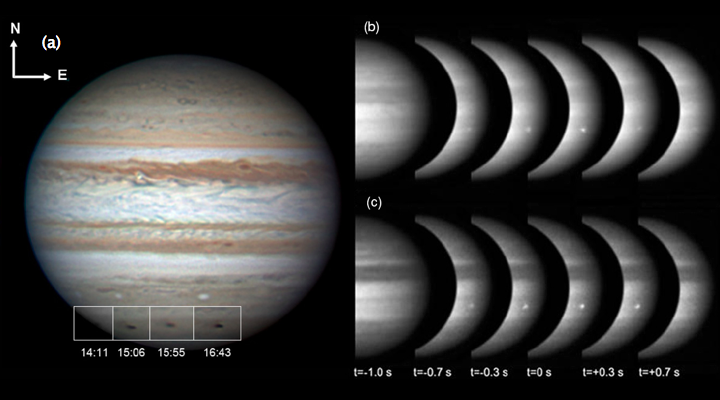
\includegraphics[width=\linewidth]{figs/jupiter-impacts.png}
\caption{Citizen science contributions to monitoring of impacts in the Jupiter
system. (a) Dark impact scar in Jupiter's atmosphere imaged by Anthony
Wesley on July 19th 2009 \citep{Sanchez-LavegaEtal2010}. (b) The
evolution of a smaller bolide impact on June 3rd 2010 at red
wavelengths, also imaged by Wesley. (c) The evolution at blue
wavelengths by Christopher Go, figure from \citet{HuesoEtal2010}.}
\label{fig:jupiter-impacts}
\end{figure}
%%%%%%%%%%%%%%%%%%%

Video monitoring has been used to enable high resolution ``lucky'' imaging of
Jupiter: the best images at moments of clear seeing from the high-resolution
video frames are selected, extracted and stacked together, using custom software
to correct for the distortions associated with the telescope optics and residual
atmospheric seeing.  Software written by citizen scientists for free
distribution to active observers, such as
Registax\footnote{www.astronomie.be/registax} and
Autostakkert\footnote{www.autostakkert.com},  allows them to process their own
video files to search for impacts in an automated way (e.g., Jupiter impact
detections\footnote{http://www.pvol.ehu.es/software/} and LunarScan from the
ALPO Lunar Meteoritic Impact
Search\footnote{http://alpo-astronomy.org/lunarupload/lunimpacts.htm}), thus
avoiding the need for transfer and storage of large datasets on some centralised
server. 
%
% Some differences become noticeable when user preferences are introduced; for
% example, use of wavelets to sharpen images can sometimes ``over-process'' the
% image, and introduce artefacts.  Colour images are put together and tuned using
% commercial packages like Adobe Photoshop, and the balance between red, green and
% blue is at the users discretion, usually with the aim of maximising contrast to
% show as many features as possible.  When such images are used for science (e.g.,
% point to point contrast measurements), it is often desirable to work with the
% raw, unprocessed images alongside the processed ones, precisely to avoid these
% artefacts and user biases.
%
The lucky imaging technique has the added benefit of providing long baseline
time-sampled observations for impact flash detection.   At least three flashes
were confirmed between 2010 and 2012, and the light curves used to determine the
sizes and frequency of objects colliding with Jupiter \citep[e.g.,][]{10hueso}
(\Fref{fig:jupiter-impacts}).  


Descriptive records of morphological changes and events are maintained and
continuously updated by organisations of citizen scientists such as the British
Astronomical Association (BAA) and the Association of Lunar and Planetary
Observers (ALPO). The BAA's Jupiter
section\footnote{http://www.britastro.org/jupiter/} is a team of amateurs with
substantial expertise in Jupiter's appearance \citep{95rogers};  Their regular
bulletins describe the changing appearance of the banded structure, the
emergence of new turbulent structures and weather phenomena, and keep a record
of the long-term atmospheric changes.  

Recent software developments have provided a much more quantitative angle on
these observations. The WinJUPOS
software\footnote{http://jupos.privat.t-online.de/} was developed by a team of
amateurs led by G. Hahn and H.-J. Mettig. It allows multiple images to be
stacked with a correction for the rapid (once per ten hour) rotation of Jupiter
or Saturn, then reprojected onto a latitude-longitude coordinate system, so that
the precise positional details of atmospheric features can be determined via
``point-and-click.''  By doing this over many nights surrounding Jupiter's
opposition, the team builds up enormous drift charts (tens of thousands of
positional measurements) for features, ranging from the tiniest convective
feature being moved by the jet streams, to the largest vortices.  The positions
can be extrapolated forward in time, enabling targeted observations by
professional observatories or even visiting spacecraft.  This long-term record
of Jupiter's visible appearance by citizen scientists has proven invaluable for
jovian atmospheric scientists.

Saturn's appearance is typically more subdued than that of Jupiter, but 20-30 cm
diameter telescopes are capable of resolving small convective cloud activity.  A
close collaboration between amateurs and Cassini spacecraft scientists allows
correlation of lightning-related radio emissions detected by the spacecraft with
visible cloud structures on the disc (known as Saturn Storm Watch)
\citep[e.g.,][]{11fischer}, which would not be possible with the targeted
regional views provided by Cassini's cameras alone.  This provides insights into
the moist convective processes thought to power the dynamics of the giant
planet, and is a good example of how citizen science can support an
international planetary mission. Amateur observations of Uranus and Neptune are
in their infancy and require telescopes with diameters exceeding 25 cm, but
there have been confirmed reports of atmospheric banding and discrete cloud
features when near-infrared filters are used to maximise contrast between white
clouds and the background and long exposure times of tens of minutes.

Active citizen observing also provides long-term monitoring in the inner solar
system.  Venus' photochemical smog shields the planet's surface from view, but
discrete cloud features can be used to study the super-rotation of the Venusian
atmosphere and the occurrence of a mysterious ultraviolet absorber high in the
planet's atmosphere (i.e., using near-UV filters).  The Venus Ground-Based Image
Active Archive was created by ESA to provide contextual observations supporting
the Venus Express mission \citep{08barentsen}.  Near-infrared imaging can be
used to sample thermal emission from the Venusian surface on the nightside
\citep{93lecacheax}. 

The Martian atmosphere, with its ephemeral clouds,
seasonal CO2 polar ice cycles and dust storms, continues to prove popular among
citizen observers, although these typically supplement the wealth of
high-resolution information being returned by orbital and surface missions to
the red planet.  As with other planetary targets, amateur observations provide
the long temporal records for the evolution of atmospheric features.  Groups
such as the International Society of Mars Observers
(ISMO\footnote{\texttt{http://www.mars.dti.ne.jp/~cmo/ISMO.html}}), the British
Astronomical Association (BAA) and the International Mars Watch program
quantitatively and qualitatively assess these amateur images. 

In \Fref{fig:planets} we show some examples of planetary images obtained
by the amateur community.

%%%%%%%%%%%%%%%%%%%
\begin{figure}[!ht]
% cp citscirev_figures.001.png planets.png
\centering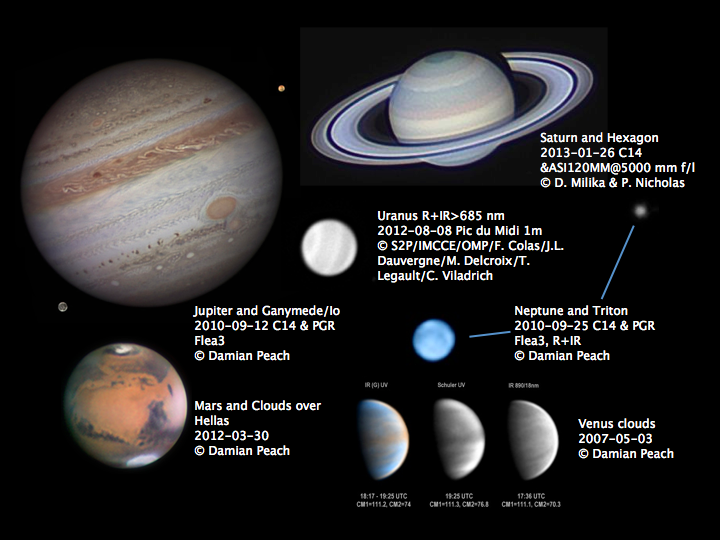
\includegraphics[width=\linewidth]{figs/planets.png}
\caption{Examples of high fidelity images obtained by amateur planet observers.}
\label{fig:planets}
\end{figure}
%%%%%%%%%%%%%%%%%%%


\CaseStudy{The International Meteor Organisation: Distributed Meteor Detection
and Tracking.} Closer to home, citizen scientists play a crucial role in the
recording of rare and unpredictable events such as the fireballs from meteoroid
impacts, such as the February 2013 Chelyabinsk meteor.  Video footage of the
fireball and shockwave were essential to scientifically characterise the
impactor and its likely origins.  \todo{Leigh}{Add refs for Chelyabinsk meteor
strike.} These reconstructed trajectories even permit the recovery of meteorites
from a strewn field (i.e., when the meteor survives the intense heat of
atmospheric entry and reaches the ground).  These objects are the remnant debris
left over from the epoch of planetary formation, and fragments left over from
comets and asteroids, so their numbers, sizes and composition provide a window
onto the earliest evolutionary stages of our solar system.  The statistics of
these impacts can only be obtained via a global network of enthusiastic citizen
scientists, sharing and publicising their observations of meteors via the
International Meteor Organisation (IMO\footnote{\texttt{http://www.imo.net}}).
\todo{Phil}{Provide high level comment on operation of IMO.}  

% Beyond Earth, transient impact flashes due to lunar impacts are recorded by
% video monitoring of the non-illuminated fraction of the Moon, aiming to
% determine the impact hazard at the lunar surface.  These quantitative studies of
% impacts in the Earth-Moon system allow scientists to understand the meteoritic
% streams threading our solar system; identify previously unrecognised meteor
% showers; and determine the statistics of potentially hazardous encounters with
% this extra-terrestrial material. \todo{Leigh}{Add refs for lunar meteorites? Or
% chop this back...}


% % -  -  -  -  -  -  -  -  -  -  -  -  -  -  -  -  -  -  -  -  -  -  -  -  -  - 
% 
% \subsubsection{Galactic and Extragalactic Observations}


\CaseStudy{Exoplanet Transits.} Beyond our solar system, amateurs have
contributed to exoplanetary transit discoveries,  attempting to measure the 1\%
diminution in starlight as a giant planet transits in front of its parent star.
\citet{13mousis} points out three methods where amateurs can contribute to
characterising exoplanetary systems ? (i) by frequent observations of known
transits to refine ephemeris; (ii) searching for transit time variations that
can reveal additional planets in a system; and (iii) searching for previously
unidentified transits in known planetary systems \citep[e.g., the discovery of
the transit of HD 80606b from a 30 cm telescope near London,][]{09fossey}.


\CaseStudy{Nearby Supernova Detection.}
\todo{Chris,Phil}{Review nearby supernovae work.}

\CaseStudy{Variable Star Monitoring: the AAVS.}
\todo{Phil}{Review variable star monitoring, AAVS.}

\CaseStudy{John Johnson's Stellar Target Selection}. An example of an amateur
expert collaborating with a professional team.
\todo{Phil}{Review Johnson et al's program.}



\todo{Chris,Leigh,Phil}{We could review how these various projects accumulate
monitoring data, and ask if this is scalable/repeatable. How does it compare to
efforts in other fields, notably ecology?}


% % - - - - - - - - - - - - - - - - - - - - - - - - - - - - - - - - - - - - - - - 
% 
% \subsection{Archive Observing (1 page)}
% \label{sec:obs:archive}
% 
% 
% \CaseStudy{Reprocessing Planetary Mission Images: UnmannedSpaceflight.com.} It
% is not just active observers who have begun using sophisticated image processing
% techniques.  There is a growing community of citizen software specialists who
% devote their time to processing of raw images from interplanetary missions,
% including those that the professional teams (i.e., those responsible for running
% the missions) simply don't have the time or resources to process completely.  
% Chief among these is the online forum, UnmannedSpaceflight.com, whose stated aim
% is to ``advance public interest in, and use of, space exploration data.''  This
% includes both raw data provided by the space agencies but not published or
% officially released (e.g., the Cassini raw data stream of images from
% Saturn\footnote{http://saturn.jpl.nasa.gov/photos/raw/} and those from the
% Curiosity rover on Mars,\footnote{
% http://mars.jpl.nasa.gov/msl/multimedia/raw/}) as well as those images
% previously released by the agencies but re-processed and colourised by dedicated
% citizen scientists.  Depending on the quality of the original, raw images, this
% can sometimes produce renderings of old data in new and startlingly beautiful
% ways.  Although not directly used for scientific enquiry, they certainly promote
% astronomy to the broader public.
% 
% \question{Chris}{Point for discussion: how hard-nosed do we want to be about
% science versus outreach in this venue? The above paragraph raised a small red
% flag with me.}
% 
% % - - - - - - - - - - - - - - - - - - - - - - - - - - - - - - - - - - - - - - - 

\subsection{Passive Observing (1 page)}
\label{sec:obs:passive}

While amateur astronomers have aquired a great deal of very useful data, the
general population is better equipped than ever to image the sky and make that
data available for scientific analysis. This has been demonstrated by two
recent professionally-led studies, that made use of a largely passive
observing community connected via online social networks not usually
associated with astronomy. 

\CaseStudy{The Orbit of Comet Holmes from the Photographs Uploaded to Flickr.}
\citet{Lang++2011} used N images scraped from the photo sharing website Flickr
as inputs to a reconstruction of the orbit of Comet Holmes. This comet was
bright enough to be visible with the naked eye in XX, 20XX, and a large number
of photographs were taken of it, and uploaded to the Flickr site.
\citeauthor{Lang++2011} were able to astrometrically calibrate the images that
contained enough detectable stars in the background using their automatic
image registration software, \texttt{astrometry.net}. This had been enabled as
a Flickr ``bot,'' crawling over all images submitted to the
\texttt{astrometry.net} group and sending the photos' owners messages showing
them where on the sky their images were taken. The calibrated images trace out
the trajectory of the comet over N nights, allowing a refinement of the
comet's orbit of ... As the authors point out ...  While in this case the
photographers did not realize they were participating in a scientific study,
the potential of combining powerful calibration software with large amounts of
citizen-supplied imaging data is made clear. 

\todo{Phil}{Finish off Lang and Hogg Comet Holmes review.}

\CaseStudy{Detecting Meteor Showers with Twitter.}
By saving a nightly (?) log of all tweets submitted to the web service
Twitter, \citet{Barentsen++2010} were able to 
detect several new meteor showers simply by searching for the text string
``meteor.'' Unwitting naked-eye observers had spotted shooting stars and
tweeted about them, giving rise to a detectable signal in the steam of tweets
that night. The detected sample is incomplete/unlocalised/ etc... However,
this work illustrates the potential both of Twitter as a communication system
for connecting large numbers of observers with a science team, and of networks
of unequipped observers for doing very bright object transient astronomy.

\todo{Phil}{Track down refernce for Barentsen twitter meteor project...}

\question{Phil,Chris}{Are there other passive observing examples? Only two so far...}


% ------------------------------------------------------------------------------

\section{Visual Classification (6 pages)}
\label{sec:class}

Observing the night sky with a telescope is perhaps the most familiar of the
activities of amateur astronomers, but as the previous section showed, citizens
are also actively involved in the processing and interpretation of the data they
have taken.  In this and the next section we look at projects where much larger
archival datasets are made available to crowds of citizens, who are asked to
inspect astronomical images, and help describe and characterize the features in
them. Despite significant advances in machine learning and computer vision, the
visual inspection of data remains an important part of astronomy, as it
continues to take advantage of the amazing human capacity for visual pattern
recognition. While many in the 1990s predicted that the increasing size of
astronomical datasets would make such time-intensive inspection impossible, the
ability of the world wide web to reach large audiences has meant the involvement
of hundreds of thousands of citizen scientists in this form of data analysis.  


% - - - - - - - - - - - - - - - - - - - - - - - - - - - - - - - - - - - - - - - 

\subsection{Visual Classification in Astronomy (3 pages)}
\label{sec:class:astro}

\CaseStudy{Stardust@home}
While significant preliminary work had been carried out by NASA's clickworkers
project (see below), the project that first illustrated the potential of
crowdsourcing for astronomical purposes was Stardust@home. This effort, which
asked volunteers to scan through images of samples returned from Comet Wild-2
by the \emph{Stardust} mission, attracted a large audience to the apparently
unprepossessing task of looking for dust grains in an effort to identify
samples of material from outside our Solar System. The site was built on
BOSSA, an early attempt to build a generalized platform for such crowdsourcing
projects (see next section), and featured a stringent test which had to be
passed before classifications were counted. Despite this hurdle, more than
20,000 people took part and a variety of dust grains were removed from the
aerogel for further study, at least one later proving an excellent candidate
for an interstellar grain. Perhaps the most significant long-term impact of
Stardust@home, though, was the demonstration that large amounts of volunteer
effort were available even for relatively `unsexy' tasks such as hunting dust
grains which do not involve intrinsically beautiful images, and that, with a
suitable website design and stringent testing, scientifically valuable results
could be obtained. 

\todo{Chris}{Add Stardust@home references...}

\todo{Chris}{Add Stardust@home url as a footnote.}

\CaseStudy{Galaxy morphology with Galaxy Zoo} 
These results directly inspired the development of Galaxy Zoo, perhaps the most
prominent scientific crowdsourcing project to date. Galaxy Zoo was built on the
continued importance of morphological classification of galaxies. First
introduced in a systematic fashion by Hubble, and later developed by amongst
others de Vaucoleurs, it remains the case that the morphology of a system is
closely related to -- but not entirely defined by -- parameters such as colour,
star formation history, dynamics, concentration and so on.  In an effort to
prepare for large surveys such as the Sloan Digital Sky Survey (SDSS), Lahav et
al. followed especially by the work of Ball et al. developed neural networks
trained on small samples of expert classifications in order to automate the
process of classification,\footnote{The Lahav papers are perhaps as interesting
for their psychology as for their astrophysics, as the classifications reveal
the relations between the senior classifiers employed to be experts} arguing
that the size of the then up-coming surveys left no place for manual
classification.

\todo{Chris}{Add real refs for automatic morphology classification}

The performance of the automatic classifiers depended on the input parameters,
including colour, magnitude and size. These variables correlate well with
morphology, but are not themselves morphological, and when included they
dominate the classification. In particularly for galaxies which do not fit the
general trends, such as spirals with dominant bulges, or star-forming
ellipticals, automated classifiers whether using these simple measures or more
complex proxies for morphology such as texture fail to match the performance
of expert classifiers. Schawinski and Nair, amongst others, spent substantial
time during their time as graduate students classifying tens of thousands of
galaxies. \todo{Chris}{Add citations showing value of Schawinski and Nair's efforts.}

Inspired by Stardust@home, a group led by one of the authors (Lintott) created
Galaxy Zoo in 2007 to provide basic classifications of SDSS
galaxies\footnote{The original Galaxy Zoo is preserved at
\texttt{http://zoo1.galaxyzoo.org} with the current incarnation at
\texttt{http://www.galaxyzoo.org}.} Classifiers were presented with a coloured
image centered on and scaled to one of more than 800,000 galaxies, and could
select from one of six options: clockwise, anti clockwise and edge-on spirals,
ellipticals, mergers and ``star/don't know.'' Aside from  an easily-passed
initial test, little knowledge was required or indeed presented to classifiers,
enabling them to proceed quickly doing something real soon after arriving at the
site; this approach, in contrast to Stardust@home where a difficult test needed
to be completed before authentic and useful contributions could be made, was
successful in encouraging large numbers of visitors to participate. This tactic
-- in which both passing and sustained engagement provide substantial
contribution -- is illustrated in \Fref{}  which shows results from Galaxy Zoo
2. \todo{Chris}{Insert box diagram illustrating Zooniverse tactics / GZ2
results.} This later version of the project asked for more detailed
classifications via a decision tree containing questions such as `How prominent
is the bulge?', and later iterations of the project have applied a similar
approach to galaxies drawn from \emph{Hubble Space Telescope} surveys including
\textsc{GEMS, GOODS, COSMOS} and \textsc{CANDELS}. 

\todo{Chris}{Add galaxy zoo participation statistics}. 

These figures are undoubtedly impressive, but they would be meaningless if the
classifications provided were not suitable for science. With sufficient effort
to ensure each galaxy is classified multiple times (as many as 80 for many
Galaxy Zoo images), these independent classifications need to be combined into a
consensus. As discussed in later sections, this can become complex but for
Galaxy Zoo a simple weighting which rewards consistency, first described in
\citet{Land++}, was sufficient. \phil{By what criteria was it sufficient?}

\todo{Chris}{Check consistency between sections: there are lots of ``see below'' type statements in this section.}

Importantly, combining classifications provides not only the assignment of a
label but, in the vote fraction in a particular category, an indication of the
reliability of the classification. This allows more subtle biases, such as the
propensity for small, faint or distant galaxies to appear as elliptical
regardless of their true morphology, to be measured and accounted for (see
Bamford et al.). The net result is that the Galaxy Zoo classifications are an
excellent match for results from expert classification, and have produced
science ranging from studies of red spirals (Masters et al.) to investigations
of spiral spin (Slosar et al.).

\todo{Chris}{Let's back up the accuracy claims here with some citations and numbers.}

A full review of Galaxy Zoo science is beyond the scope of this review; a
recent summary is given in the Galaxy Zoo 2 data release paper by Willett et
al. However, it is worth noting that many of the project's most important
results have been the result not of interaction with the main interface but
represent rather serendipitous discoveries made by participants. We return to
these in Section~\ref{sec:explore} below.

\question{Chris}{How much GZ science do we want to cite? Some key/high impact papers would be good, I think. There is currently a difference in emphasis and style between this section and Leigh's observing sections, that we ought to work to reduce (perhaps on both ends). Leigh gives lists of results with very short introductions; this section tells a more involved story of one project. Let's discuss how to resolve this.}


\CaseStudy{Surfaces of solar system bodies: Moon Zoo, Moonwatch.}

If studying galaxies remains, at least in part, a visual pursuit, then the same
is certainly true of planetary science. NASA's clickworkers, which asked
volunteers to identify craters on the Martian surface, lays claim to be the
oldest astronomical crowdsourcing project. The consensus results matched those
available from experts at the time, but failed to go beyond this promising start
to produce results of real scientific value. More recently, interfaces inviting
classifiers to look at the Moon, Mercury, Mars and Vesta have been launched and
attracted significant numbers of classifications, but although preliminary
results have been promising these projects have yet to produce datasets that
have been used by the planetary science community in the same way that Galaxy
Zoo has by the astronomical community. 

\todo{Chris}{Fact-check the consensus with experts claim about clickworkers.}

\todo{Chris}{Provide clickworkers reference.}

\chris{Is this too negative? I wanted to go on to say lots about the need for
serious effort to make use of classifications, but felt it was perhaps better
to leave it there and move on.}
\phil{I think it's fine like this. Do they have any papers to cite at all? We could at least give the urls in footnotes.}

\todo{Chris}{Tidy up the multiple mentions of clickworkers. Whats the optimal ordering of these sections given their inter-references?}


\CaseStudy{Time domain astronomy: Supernova Zoo and Planet Hunters}

If citizen science is to be a way of dealing with ``Big Data'' then it is
perhaps useful to remember that data sets can be big enough to be problematic in
a variety of ways; the XXXX CITE XXXX describes the `three Vs'' of Big Data -
volume, velocity and variety. Time-domain astronomy projects requiring the
immediate inspection of challenging  volumes of live data can also benefit from
citizen science. While transients such as supernovae or asteroids can often be
found through the use of automatic routines, visual inspection is still used by
many teams as part of the process of selecting candidates for follow-up. 

\todo{Chris}{Citation for expert visual classification of supernova candidates? SDSS SN search?}

The most successful attempt to use crowdsourcing to attack these problems to
date has been the offshoot of Galaxy Zoo described in Smith et al, ``Supernova
Zoo.'' Data from the Palomar Transient Factory XXX CITE XXX was automatically
processed and images of candidate supernovae uploaded on a nightly basis; this
triggered an email to volunteers who, upon responding were shown the new image,
a reference image and the subtraction between the two. By analyzing the answers
to a series of questions, candidates were sorted into three categories, roughly
corresponding to ``probable supernova,'' ``likely astrophysical but
non-supernova transient'' and ``artifact.'' The results were displayed on a
webpage and used to select targets for follow-up. Despite the site attracting
many fewer classifiers than the main Galaxy Zoo, it was highly effective in
sorting through data, with consensus typically reached on all images within 15
minutes of the initial email being sent. 

\todo{Chris}{Add SN zoo, PTF refs}

\question{Chris}{We should review Richards and Blooms' work using the SN zoo data to improve the automated analysis -- this is an important application of citizen science results, no? Where does it belong though? Here is just the place it happened to come up -- but it could have been anywhere, I think.}

\question{Chris}{Is this the right place to discuss ideas for future time domain astronomy projects with LSST? Or shall we postpone that to a ``future'' section?}

Archive projects such as the main Galaxy Zoo have the luxury of being able to be
inefficient.  \phil{This made me frown. it's bad to be inefficient when we are
talking about peoples time! Can we re-direct this somehow? I'm not sure this part belongs in time domain astronomy: don't we want to improve efficiency in all projects?} When the appetite of
volunteers for classification is high, and little of consequence is attached to
finishing the task in, for example, three months instead of six, there is little
incentive to direct attention efficiently. A random assignment of task to
classifier thus, in most cases, suffices, but this is not true when rapid
classification is important (or in the case of larger datasets). Using the
supernova project's archive as a test, Simpson et al. developed a Bayesian
method for assessing classifier performance; in this view, each classification
provides information both about the subject of the classification and about the
classifier themselves. Classifier performance given subject properties can thus
be predicted and an optimum set of task assignments calculated. For systems
involving tens of thousands of classifiers and perhaps a similar volume of
subjects to be classified, an exact solution is computationally extremely
expensive, but a MCMC approach can be used to find efficient solutions. Work by
Simpson et al., as well as Horvitz et al and Waterhouse on Galaxy Zoo data,
suggests that accuracy can be maintained with as few as 30\% of classifications.
This sort of optimization will be increasingly important for online citizen
science, but a major challenge (\phil{What sort of challenge?}) remains in
incorporating this sort of analysis in live systems rather than using archive
data. 

\todo{Phil}{Add reference to Space Warps, and planned online/real time extension here?}

\todo{Chris}{Bibtex references!}

\todo{Phil,Chris}{Discuss where to put section on increasing efficiency through classifier analysis}

A different approach to time-domain astronomy through citizen science is
exemplified by the Planet Hunters project, which asks volunteers to examine
light curves drawn from the dataset provided by the \emph{Kepler} mission in
order to identify interesting events in retrospect. While the task of
identifying transits from extrasolar planets is, at first glance, one which
seems more suited for automated than for human analysis, the success of Planet
Hunters in identifying more than fifty planet candidates missed by the
automatic routines suggests that there remains a role for inspection by eye in
cases where the relevant science requires completeness of classifications.
While several of the planets found by Planet Hunters, including the project's
first confirmed planet (PH1b, Schwamb et al.), are unusual 
-- PH1b, a
circumbinary, is the first planet known in a four-star system --  others,
including the more than forty candidates identified in the habitable zone of
their parent star by Ji et al., might have been expected to be recovered by
more conventional searches. Planet Hunters, therefore, is acting as an
independent test of the Kepler pipeline's efficiency (Schwamb et al.) and has
inspired improvements in subsequent analysis (Bathalia et al.). More recently,
advanced users have participated in the identification of unusual stellar
properties - see XXXXXXXX. 

\question{Leigh}{Are there any visual classification activities going on in solar system science that belong in this section rather than anywhere else? They needn't be based around pupose-built websites like Galaxy Zoo, but if the product of them is visual classification data we might include them here for contrast. I guess there is visual classification going on in the
rapid-reaction events (jovian/lunar impacts, storm/plume eruptions) described in the observing section -- but how are those classifications collected and analyzed? Is there any systematic analysis of the crowd's outputs?}

\question{Leigh}{I also have a note here that says ``Data mining for asteroids
and TNOs'' - know anything about that?}

\question{Chris}{Are there any other astronomical classification-based citizen
science projects we should review? Planet 4? Non-Zooniverse projects?}

% - - - - - - - - - - - - - - - - - - - - - - - - - - - - - - - - - - - - - - - 

\subsection{Visual Classification in Other Fields (\textbf{Chris}, Phil, 1 page)}
\label{sec:class:non-astro}

Although, as described in the previous section, astronomical analysis led the
development of citizen science as a data analysis tool, it has quickly been
adopted by other fields. In some cases, this adoption has been explicit. The
tools developed for Stardust@home were developed into a general purpose
library for citizen science, BOSSA, which has recently been ported to python
as PyBOSSA, and the Zooniverse platform which supports many of the examples
described above includes projects from fields as diverse as ecology and
papyrology. This diversity of projects allows general lessons about project
design to be drawn; indeed, this is an active area of research for academic
fields as diverse as computer science, economics and social science. 

\todo{Chris}{Add citation to Crowston paper on PH and Seafloor Explorer}

Perhaps the most important result from such studies is the beginnings of an
understanding of participant motivations. Perhaps surprisingly, the
participants in online data analysis citizen science projects are to a large
extent a distinct community from those who participate in more traditional
amateur astronomical activities; Galaxy Zoo classifiers, for example, are not
for the most part regular observers. Initial work by Raddick et al. showed
that the primary motivation of such communities is to assist science, a choice
which was much more popular than alternatives including a preexisting interest
in astronomy or a desire to see more beautiful images\footnote{Given the
advent of projects such as Planet Hunters which involve looking at graphs
rather than images, perhaps this is just as well!}. 

\phil{We have a whole subsection on motivation in the ``demographics'' section later on -- I think we should postpone the above paragraph to then.}

Projects from other fields can also suggest strategies which could be adopted
by future astronomical projects. In particular, future projects involving
analysis of survey data which has been collected for a multitude of purposes
may require a more sophisticated model for data analysis than the simple
decision tree presented by projects such as Galaxy Zoo. Snapshot Serengeti, a
Zooniverse project which analyses images from more than two hundred
motion-sensitive ``camera traps,'' offers a particularly sophisticated response.
Driven in part by the need for an interface which allows volunteers to state
the obvious (for example, identifying elephants, lion or zebra) and also to
provide more obscure classification (for example, distinguishing between types
of gazelle), a variety of classification paths are presented. In addition to
just clicking buttons identifying species, volunteers can opt for a decision
tree-like approach, or choose from a variety of similar species (``Looks like
an antelope...'') or search the descriptions provided (``Show me all animals
whose descriptions involve 'ears' ''). This hybrid model has proved successful
not only in encouraging classification, but also in encouraging learning; over
a Snapshot Serengeti classifier's ``career'' they are increasingly likely to
chose more direct routes.

\todo{Chris}{Include Snapshot Serengeti citations}

\phil{Is the SS experience relevant to open ended exploration of survey images?
I've wondered for a while whether diagnosis of astronomical image reduction
problems could be done by crowd-sourcing: DES do a lot of visual inspection just
within their team, LSST could serve a larger volume to more people, potentially.
The viewer ubrets with their shareable URLs seem vital for this; might SS-style
interfaces also be important?}

Another design area in which non-astronomical projects have much to teach us
is that of ``gamification'' -- the inclusion, either
explicitly or implicitly, of game-like mechanics such as scores, ``badges'' or
other rewards, leader boards, and so on, in the classification process.

\todo{Chris,Phil}{Include discussion of one or two non-astronomy citizen science projects that include gamification. Fold.It? Others? What do these projects know about the impact of their design choices? We should review the debate, with citations to papers.}

An early experiment with Galaxy Zoo showed that the addition of a score
dis-incentivised poor classifiers, but also resulted in the best classifiers
leaving, presumably having been satisfied once a top score was achieved. A
recent study by Eveleigh et al. of the Old Weather project, which included
basic rankings for classifiers, highlighted these dangers, identifying
volunteers who were alienated by the addition of this game-like score, feeling
discouraged when top scores could not be matched, or worrying about data
quality if the scoring scheme rewarded quantity of classifications rather tham
accuracy. Taking seriously the finding described above that citizen scientists
are motivated by a perception of authentic participation in research, it seems
right to be cautious about introducing elements which are or which are
perceived to be in tension with this primary motivation. 

\phil{This is an important statement to make. However, we only review the motivations of users later on, in the demographics section -- so e have to think a bit about what belongs where. The trickiness comes form this being an ``ideas'' section, I think -- we have somehow ended up not just reviewing what has been done, but arguing a case for doing something different. }

Furthermore, the
introduction of a significant incentivizing scheme relies on an accurate model
of what `correct' behaviour would look like; this may prove a significant
barrier both to accuracy if such a model is not available (for example, in
Planet Hunters such a model would not have included unusual systems such as
PH1b) and, where a strong incentive scheme results in near-uniform classifier
behaviour, a loss of flexibility in later data analysis. 

These caveats aside, there are examples of projects which have successfully
incorporated gamified elements into their design. Perhaps the most successful
is Eyewire, a project based at MIT which seeks to supplement machine learning
identification of neurons in three-dimensional scans. Participants in the
project, who are asked to identify connected regions throughout a
three-dimensional scan, earn points based on participation and also have a
separate, publicly visible, accuracy score. 

\phil{If Space Warps' SWAP analysis goes live, we could easily display the agent ``skill'' on the volunteer's profile page...}

In addition to overall leader
boards, the project also runs short challenges including a regular Friday
``happy hour'' in which participants compete on specific problems. Eyewire is
also notable for its strong community elements, with a chat room open and
available to all participants in the project (supplemented, incidentally, by a
``bot'' built by a participant which answers frequently asked questions from new
users). 

\phil{I wish we could cite the Zoonibot!}

A strong comparison of the type of reward structure utilized by
Eyewire and the approach used by more traditional projects such as Galaxy Zoo
is urgently needed in order to inform future project design. 


% ------------------------------------------------------------------------------

\section{Data Modeling: Citizen Analysts (4 pages)}
\label{sec:model}

New understanding of the world comes from the interpretation of data in the
context of a model. The modeling activity itself often has technical
difficulties that computers may find hard to overcome, associated with complex
and/or computationally expensive, likelihood functions. Humans, by applying
their developed intuition, can often contribute a great deal to the
exploration of a model's parameter space by closing in quickly on the model
configurations that are fit the data well. This process can be particularly
satisfying, rather like solving a puzzle. How have citizen scientists been
involved in model making and data fitting in astronomy, to date?


% - - - - - - - - - - - - - - - - - - - - - - - - - - - - - - - - - - - - - - - 

\subsection{Data Modeling in Astronomy (2 pages)}
\label{sec:model:astro}

A number of  web-based citizen astronomy projects include an element of data
modeling as part of their set tasks. 

\todo{Phil}{One or two more sentences about what the hell data modeling is?}

\CaseStudy{The Milky Way Project}
\citet{SimpsonEtal2012} provided volunteers with a fairly flexible set of
annulus-drawing tools, for annotating circularly-symmetric ``bubble'' features
in colour-composite (24.0, 8.0 and  4.5$\mu$m) infrared images from surveys
carried out by the Spitzer space telescope, which are hypothesised to have
been caused by a recently-formed high mass star at the centre of the bubble.
The (bubble) model in this case is simple and recognisable, making both the
interface constructions and its operation relatively straightforward. The
large sample of  bubble models have been used to investigate the possibility
of further star formation being triggered at the bubble surfaces
\citep{KendrewEtal2012}.

% Another Zooniverse project, Space
% Warps,\footnote{\texttt{http://spacewarps.org}} also involves data modeling,
% but not directly on the interface, which is restricted to enabling
% identification (``spotting'') gravitational lensed images. A fraction of the
% community is engaged in modeling the  identified lens candidates using
% web-based software developed and supported  by the science
% team.\footnote{\texttt{Lens Labs}} 

\todo{Phil}{Add text on modeling in Space Warps. No Letter, but an extensive Talk discussion board, and Rafi's paper (on modeling the Space Warps sims with SpaghettiLens) should be out soon...}

\CaseStudy{Galaxy Zoo: Mergers} This has been perhaps the most advanced attempt
at data modeling in  astronomical web-based citizen science
\citep{HolincheckEtal2010,WallinEtal2010}. (\question{Chris}{Is this statement
still true? Good if you can check through this case study...} Here, simple
N-body simulations of galaxy mergers were performed in a java applet, and the
results selected according to visual similarity to images of galaxy mergers
(previously identified in the Galaxy Zoo project). A key proposal in this
project is that the inspectors of the simulation outputs would be able to find
matches to the data more readily than a computer could, for two reasons. First
is that humans are good at {\it vague} pattern matching: they do not get
distracted by detailed pixel value comparisons but instead have an intuitive
understanding of when one object is ``like'' another. The second is that
initialising a galaxy merger simulation requires a large number of parameters to
be set -- and its this high dimensionality  that makes the space of possible
models hard to explore for a machine. Humans should be able to navigate the
space using their intuition, which is partly physical and partly learned from
experience gained from playing with the system. Initial tests on Arp 86  showed
the crowd converging on a single location in parameter space, and that the
simulated mergers at this location do indeed strongly resemble the Arp 86
system. The authors have since collected thousands of citizen-generated models
for a sample of a large number SDSS merging systems (Holincheck et al, in
preparation). 

\todo{Phil}{Follow up merger zoo papers}

% %%%%%%%%%%%%%%%%%%%
% \begin{figure}[!ht]
% \begin{minipage}{\linewidth}
%   \begin{minipage}{0.45\linewidth}
%     \centering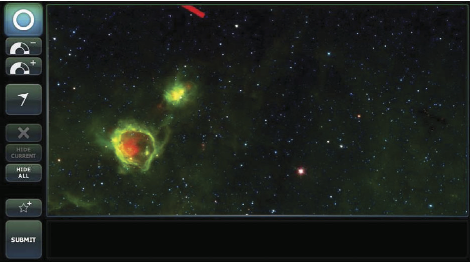
\includegraphics[width=\linewidth]{figs/SimpsonEtal2012_interface.png}
%   \end{minipage}\hfill
%   \begin{minipage}{0.51\linewidth}
%     \centering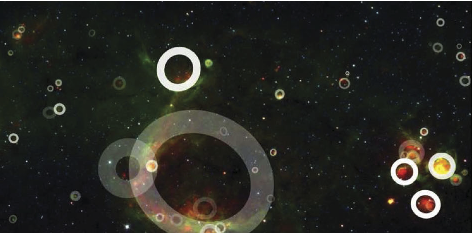
\includegraphics[width=\linewidth]{figs/SimpsonEtal2012_bubbles.png}
%   \end{minipage}\hfill
% \end{minipage}
% \medskip
% 
% \begin{minipage}{\linewidth}
%   \begin{minipage}{0.48\linewidth}
%     \centering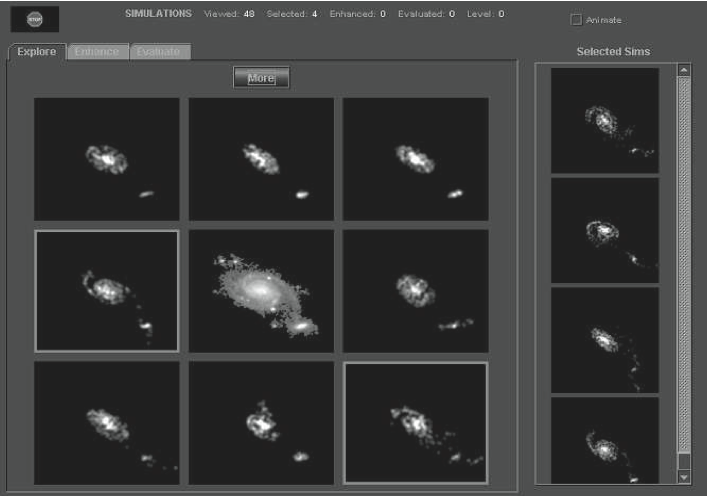
\includegraphics[width=\linewidth]{figs/HolincheckEtal2010_comparing.png}
%   \end{minipage}\hfill
%   \begin{minipage}{0.48\linewidth}
%     \centering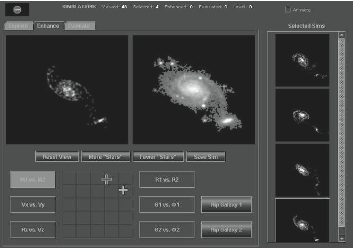
\includegraphics[width=\linewidth]{figs/HolincheckEtal2010_enhancing.png}
%   \end{minipage}\hfill
% \end{minipage}
% \caption{Examples of image modeling in web-based citizen science projects. Top
% row: star formation ``bubble'' identification and interpretation in Spitzer
% images in the Milky Way Project, with the annotation interface shown on the
% left, and some example (selected, averaged) bubbles on the right. Images from
% \citet{SimpsonEtal2012}. Bottom row: matching N-body simulated merging
% galaxies to SDSS images in the Galaxy Zoo Mergers project (left), and
% exploring parameter space two parameters at a time to refine the models
% (right). Screenshots from \citet{HolincheckEtal2010}.}
% \label{fig:modeling}
% \end{figure}
% %%%%%%%%%%%%%%%%%%%

%%%%%%%%%%%%%%%%%%%
\begin{figure}[!ht]
% cp citscirev_figures.003.png modeling.png
\centering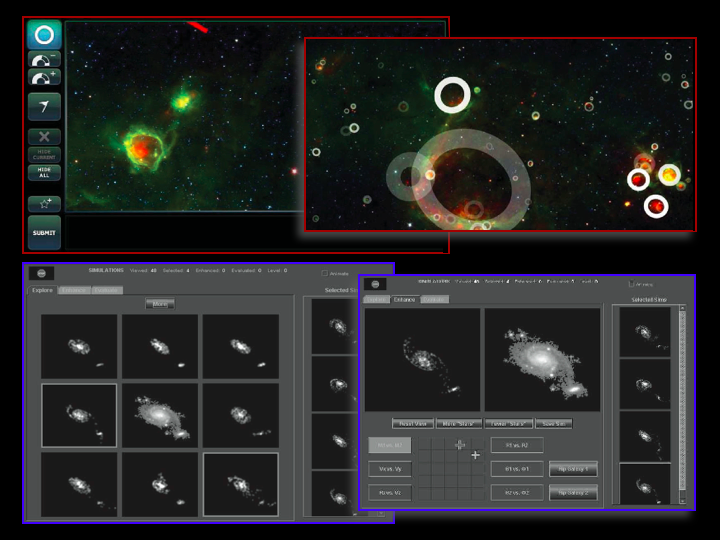
\includegraphics[width=\linewidth]{figs/modeling.png}
\caption{Examples of image modeling in web-based citizen science projects. Top
row: star formation ``bubble'' identification and interpretation in Spitzer
images in the Milky Way Project, with the annotation interface shown on the
left, and some example (selected, averaged) bubbles on the right. Images from
\citet{SimpsonEtal2012}. Bottom row: matching N-body simulated merging
galaxies to SDSS images in the Galaxy Zoo Mergers project (left), and
exploring parameter space two parameters at a time to refine the models
(right). Screenshots from \citet{HolincheckEtal2010}.}
\label{fig:modeling}
\end{figure}
%%%%%%%%%%%%%%%%%%%


The above examples involved modeling infrastructure provided by either the
project's developers or science teams. There have also been cases where
citizens have carried out modeling analyses using their own tools, or writing
their own software. For example, in the PlanetHunters project, a small group
[?] of volunteers downloaded full Kepler lightcurve datasets for the best [?]
community-selected candidates, and fitted transit lightcurves to them using
[?]. 

\question{Chris}{Is the PH forum analysis worthy of a case study here? What did the super-users actually do in th eway of advanced lightcurve modeling?}

\CaseStudy{Weak Lensing Data Challenges}
Another very interesting case is that of the analysis challenges organised by
the professional cosmology community.  The measurement of weak gravitational
lensing by large scale structure (``cosmic shear'') relies on the measurement
of the shapes of distant, faint galaxies with extreme accuracy. The STEP
\citep{HeymansEtal2006,MasseyEtal2007} and GREAT
\citep{BridleEtal2010,KitchingEtal2012,KitchingEtal2013a} blind galaxy shape
estimation challenges have had an enormous impact on the field, revealing
biases present in existing techniques, and providing a way for researchers
outside the world of professional cosmology to participate. In particular, the
GREAT08 challenge saw very successful entries (including the winner) from two
(out of a total of 11) teams of researchers from outside the field (albeit
still professional researchers). A companion, somewhat streamlined galaxy
shape measurement challenge, ``Mapping Dark Matter,'' which was hosted at the
Kaggle website\footnote{\texttt{http://www.kaggle.com/c/mdm}} 
\citep{KitchingEtal2013b}. The wider reach of this platform led to over 70
teams making over 700 entries to the competition; many of the teams did not
contain professional astronomers, although most were still from academia.
In a comparison with the
GREAT challenges, the authors found a factor of several improvement in shear
accuracy over comparable previous challenges. \citet{KitchingEtal2013b}
suggest two interesting explanations for the success of the Kaggle challenge.
First, the challenge was designed to be as accessible as possible, with an
extensive training set of data that needed very little explanation; in this
way the challenge was geared towards {\it idea generation}. Second, they note
that the competitive  nature of the challenge (a webpage leaderboard was
updated in real time as entries were submitted) seemed to stimulate the
analysts into improving their submissions. Kaggle offers cash prizes, which
will have had some effect as well (the pot
was \$3000 for this challenge, even if indirectly).

A second astronomical Kaggle challenge involved inferring the positions of
dark matter halos based on their weak lensing effects (``Dark
Worlds,''\footnote{\texttt{http://www.kaggle.com/c/DarkWorlds}} Harvey et al,
in prep.) This challenge attracted the attention of 357 teams, perhaps due to
its larger prizes. It also sparked some debate in its forums as to the design
of the challenge: the models used to generate the data, the size of the test
datasets (and consequent stability of the leaderboard),  the choice of
leaderboard metric and so on. These issues are also of generic importance for
scientists looking to crowd-source algorithm development. It is interesting to
note that the Kaggle forums are a useful resource for the Kaggle development
team: the citizens who are active there do influence the design of the site
infrastructure and challenge rules (D.~Harvey, priv.~comm.).

\todo{Phil}{Update Kaggle challenge references -- Harvey paper.}

% - - - - - - - - - - - - - - - - - - - - - - - - - - - - - - - - - - - - - - - 
% 
% \subsection{Data Modeling in Other Fields (2 pages)}
% \label{sec:model:astro}
% 
% Case studies:
% \begin{itemize}
% \item Protein folding with Fold.it. Gamification as a technique.
% \item Other examples? 
% \end{itemize}

\question{Chris}{Does Fold.It belong here, in a subsection on Data Modeling in
Other fields? And if so, whence the discussion of gamification?}

 
% ------------------------------------------------------------------------------

\section{Citizen-led Enquiry (3 pages)}
\label{sec:explore}

The previous sections have focused on specific, and isolated, activities in
which citizens have participated. In most cases, the community's involvement has
been a {\it contribution} to a scientific investigation, while not being
involved in the design of that investigation. The most important part of any
scientific investigation is the question at its heart: what is it we are trying
to find out about the universe? In this section we look at some cases where the
process of enquiry, the science, has been instigated or led by citizens.  

In principle, this is an area of great potential. The constraints of funding
proposals and management of research groups can often mean that professional
scientists focus very narrowly on particular topics of research, using a
particular technique for which they become known.  Steering away from this
course implies taking risks with time management, and allocation of resources to
an ultimately fruitless research area can be detrimental to careers.  Citizen
scientists are largely free of these managerial and budgetary constraints, and
are able to devote their attentions to whatever topics interest them: we might
expect outsiders to ask some unusual questions, and make connections and
suggestions that highly focused professionals may not have thought of. What are
some enquiries that citizens have led in astronomy to date, and how have they
been enabled and supported?


\CaseStudy{Saturn Storm Watch.} 
In this project, Cassini's observations of lightning emissions are connected
with active amateur observations of convective cloud structures within the giant
planet atmosphere; and the tracking of the vertices of Saturn's bizarre north
polar hexagon \citep{88godfrey}, a 6-sided planet encircling wave that has
persisted for at least 30 years but that has only recently been observed, by
amateur astronomers.  In the first case, citizen scientists wished to identify
the source of Saturn's radio emissions.  In the latter case, the long-term
evolution of the hexagon vertices is being used to understand what sort of wave
this is, and to identify its origins.

\CaseStudy{Online Observing} 
The Faulkes telescope is an excellent example of a facility enabling  citizen-led
enquiry: both student-devised and teacher-led investigations can be performed at
the network of robotic observatories in Hawaii and Australia, allowing students
to develop scientific questions using their own data and collaboration with
other students around the world.  A selection of some of these projects can be
found on the observatory
website.\footnote{\texttt{http://www.faulkes-telescope.com/showcases/schools}}. 
Other observatories around the world have telescopes devoted to citizen enquiry:
the Pic-du-Midi observatory\footnote{http://www.obs-mip.fr/pic-du-midi} in the
French Pyrenees has a 0.6-m telescope devoted to amateur observers.   For
example, in 2013 M.~Delacroix used the 1-m observatory to image details on
Uranus and
Neptune\footnote{http://www.cloudynights.com/ubbthreads/showflat.php/Cat/0/Number/5955129/page/0/view/collapsed/sb/5/o/all/fpart/1/vc/1}.
\phil{1-m or 0.6m? Mention Bradford Telescope.}.

\question{Chris}{Is there enough to review in this ``online observing'' section?
Seems maybe pro,ising, but we could do with some success stories to review, and
\emph{cite.}}


\CaseStudy{The Galaxy Zoo Forum.} The best known serendipitous discovery
emerging from the Galaxy Zoo project is ``Hanny's Voorwerp'' (Lintott et al.), a
galaxy-scale light echo which reveals a recent ($\sim 100000$ years) shutdown of
AGN activity in IC 2497, the neighboring spiral galaxy. The discovery of the
Voorwerp was first recorded in the Galaxy Zoo forum a few weeks after the
project started, and inspired a more systematic search for similar phenomena in
other galaxies. This project, made possible by the deep engagement of Galaxy Zoo
science team member Bill Keel in the forum community, succeeding in finding more
than forty instances of clouds which appear to have been ionized by AGN
activity, in systems a third of which show signs of significant drops in
activity on a timescale of tens of thousands of years. \todo{Chris}{Add more
citations for voorwerp science?}

The ability of the Zoo volunteers to carry out their own research, moving far
beyond the mere ``clockwork'' required by the main interface, is best
illustrated by the discovery of the Galaxy Zoo Peas. These small, round and, in
SDSS imaging, green systems are dwarf systems with specific star formation rates
(SFR per unit mass) which are unprecedented in the local Universe, matched only
by high-redshift Lyman-break galaxies. Volunteers not only identified these
systems, but organized a systematic search and further review of them, including
using tools designed by SDSS for professional astronomers to acquire and study
spectral data. 

The discovery of the Peas marked the first time the Galaxy Zoo team realized the
potential of the community of citizen scientists the project had acquired, but
it is important to note that the simpler, initial interaction provided by the
main interface was necessary in order to develop that community in the first
place. The participants in the citizen scientists' investigation of the Peas did
not arrive on the site wanting to dig into spectra or confident of their ability
to do so; these were the results of their participation. The project  acted as
an ``engine of motivation'' in inspiring its participants to become more
involved. 


Participants in citizen science projects like Galaxy Zoo and Saturn Storm Watch 
are highly motivated but geographically widely distributed; the impact of the
internet in enabling them to find each other and collaborate is remarkable. The
most recent Zooniverse astronomy project, Galaxy Zoo: Quench, is actively
encouraging citizen-led enquiry, by providing flexible tools for investigating
not individual objects but samples of galaxies classified in the main Galaxy Zoo
project. It is an experiment in citizen-driven scientific investigation, and we
await its results with interest.

\todo{Someone}{Follow up Galaxy Zoo Quench...}

% \CaseStudy{Quench}
% 
% \CaseStudy{BAA Deep Sky Observers: variable nebulae}
% 
% \CaseStudy{Amateur asteroid observations and follow-up.}

\question{Chris}{In principle there is a whole body of citizen-led research we
could review, published in the BAA magazine and elsewhere. What shall we do
about this?}


% ------------------------------------------------------------------------------

\section{Understanding the Citizens (2 pages)}
\label{sec:crowd}

Having surveyed some of the activities involving citizen scientists, we can
now consider some questions about this community itself. Who participates in
citizen science, and what motivates them?


% - - - - - - - - - - - - - - - - - - - - - - - - - - - - - - - - - - - - - - - 

\subsection{Demographics}
\label{sec:crowd:demographics}

Who is participating in citizen astronomy? We might expect the demographics to
vary with activity, and with the level of commitment required. We have some
understanding of at least the former division from two studies that were
carried out approximately simultaneously, one of the community  participating
in Galaxy Zoo, and another of the  American Association of Variable Star
Observers (AAVSO).  \citet{Rad++13} surveyed the Galaxy Zoo volunteer
community to investigate their motivations (\Sref{sec:crowd:motivation}
below), via a voluntary online questionnaire. The 11,000 self-selected Galaxy
Zoo users identified as 80\% male, with both genders having an approximately
uniform distribution in age between their mid-twenties and late fifties. The
authors point out that this is close to the US internet user age distribution,
except for slight but significant excesses in numbers of post-50s males,
post-retirement people of both genders, and a deficit in males under 30. The
survey respondents  also tended to be more highly educated than average US
internet users, with most holding at least an undergraduate degree, and around
a quarter having a masters or doctorate. 

These findings can be compared with a survey of the members of AAVSO:
\citet{P+P2012} received over 600 responses  (corresponding to about a quarter
of the community of observers and society members). The education levels of
the AAVSO repondents matches the Galaxy Zoo community very closely; the AAVSO
age distribution is more peaked (in the mid fifties), with a similar post-60
decline but also a marked absence of younger people. The online nature of the
Galaxy Zoo project seems to have increased the participation of younger (pre
middle-age) people. Likewise, the Galaxy Zoo gender bias, while itself
extreme, is less so than at AAVSO, where some 92\% of survey respondents were
male. One additional piece of information provided by the AAVSO survey is the
profession of the variable star observers: most (nearly 60\%) of the survey
respondents were found to be working in science, computer science, engineering
and education.

The Galaxy Zoo and AAVSO communities differ by more than just the nature of
their activity. The smaller AAVSO community is arguably more engaged in its
research, in the sense that a larger fraction of its membership is active in
taking observations and contributing to analyses. It would be very interesting
to know how citizen scientist motivation varied with the level of
participation: dividing the Galaxy Zoo community into volunteers that
contribute to the  forum and those who don't could be interesting; perhaps
more so would be to repeat the analysis of \citeauthor{Rad++2013} over a wide
range of projects, and look for trends there. The emergent picture thus far,
however, is of a well-educated (and often scientifically trained)  but
male-dominated citizen science community, whose female and younger membership
is likely to have been, at least in part, enabled via projects being hosted
online. Continuing to lower the barriers to entry for currently
under-represented demographic groups would seem both important, and within
reach.

\question{Chris}{Are you or anyone else on the Zooniverse team aware of
additional studies of citizen crowd composition?}


% - - - - - - - - - - - - - - - - - - - - - - - - - - - - - - - - - - - - - - - 

\subsection{Motivation}
\label{sec:crowd:motivation}

What motivates citizen scientists? The two demographic studies referred to
above also covered this question; it was the primary motivation for
\citeauthor{Rad++2013}. Having previously identified 12 categories of
motivation in an earlier pilot study \citep{Rad++2010}, \citeauthor{Rad++2013}
asked the 170,000 volunteers at the time to comment on how motivated they were
by each of these categories, and which was their primary motivation. The 6\%
who responded gave consistent answers to around 900 forum users who responded
in a separate appeal, allowing us to draw conclusions about this presumably
more engaged sub-population. A desire to {\it contribute} to science was found
to be the dominant primary motivation, being selected by 40\% of respondents.
{\it Astronomy}, {\it science}, {\it vastness}, {\it beauty} and 
{\it discovery} were all motivation categories that were found to very
important to the volunteers, while {\it fun}, {\it learning} and {\it
community} were less important. 

The AAVSO demographic survey \citep{P+P2012} found similar results: over a
third of variable star observers cited involvement in science and research as
their primary source of motivation. However, a similar number gave an interest
in variable stars as theirs, perhaps reflecting a stronger focus on the
science questions involved than is present in the Galaxy Zoo community. Both
groups of citizen scientists are clearly quite serious in their reasons for
taking part: their motivations are actually very close to those of
professional scientists, as many readers of this review will recognize.

These surveys reveal a community of people many of whom may have left  
academic science behind as soon as they finished their  education, but who
still maintained a passion for astronomy and the  boundaries of knowledge. 
Their thirst for knew information, and the  desire to be part of the 
scientific process drives them to actively observe the  night sky or to
participate in analysis of large datasets.  

For the more motivated people involved in citizen science, being part of a
community, 
albeit a distributed one, that brings great enjoyment and satisfaction.  With
the connectivity of the internet, there is a social  aspect of citizen science
that unites people with shared interests.   These pastimes and hobbies are
often far removed from someone's ``normal''  life. However, {\it community}
was not found to be a strong motivator for the Galaxy Zoo volunteers -- but it
is nevertheless very important for the Galaxy Zoo forum users. More recent
Zooniverse projects have sought to widen participation in community
discussion, hypothesizing not that it will motivate people better, but because
it will help them make better contributions. Citizen scientists, like
professional scientists, are primarily motivated by getting science done.

\todo{Phil}{Update the motivation section with any latest results. Ask teh
Zooniverse team.}



% ------------------------------------------------------------------------------

\todo{Phil,Chris}{Look at the future section together, plan it based on review
so far. What are the key themes? Focus on them?}



\section{Ideas for the future (4 pages)}
\label{sec:future}

Speculation on what will be a) made possible by advances in technology and
dataset size/availability, and b) feasible.

% - - - - - - - - - - - - - - - - - - - - - - - - - - - - - - - - - - - - - - - 

\subsection{Observations and Instrumentation in the future}
\label{sec:future:obs}

% Robotic or automated telescopes to feed data to amateur processors/users for
% immediate analysis.  Long term baselines with the same 
% instrument/calibration.
% 
% Global telescope networks for continuous monitoring.
% Distributed stations and networks for stellar occultations by TNOs and KBOs. 
% Mobile observing stations and international coordination?
% 
% Video monitoring for meteors from multiple interlinked stations for 3D
% trajectory reconstruction.
% 
% Amateur observing follows professional:
% \begin{itemize}
% \item Deeper field for amateur observations of Uranus and Neptune, particularly
% near-IR.
% \item Visible-light and near-IR spectroscopy; long-term datasets, serious
% photometry.  Calibration, calibration, calibration...
% \item Advanced technologies such as AO for image stabilisation?
% \end{itemize}
% 
% Adoption of uniform standards for amateur imaging to be provided to online
% databases (already underway with PVOL).


Today, the crucial benefits of active citizen observing are that of time and
coverage, enabled by a global network of passionate and talented observers,
connected and sharing their contributions via the internet.  The professional
community, restricted to the over-burdened resources of space observatories
and ground-based facilities, do not have the capability to replace this
contribution. Furthermore, would we want to?  After all, the close connection
between professional and amateur communities has broadened the audience for
scientific discoveries, and allowed us to use astronomy to educate and enthuse
the next generation of budding citizen scientists.  This two-way highway is a
key benefit of our present era of citizen astronomy.  However, citizen
scientists currently do this for fun and education, and professionals should
be wary of demanding more standardised, calibrated and uniform techniques for
temporal and spatial monitoring, as enthusiasm may wane if this begins to
sound like 'work' rather than a hobby.

Sadly, future advances in technology may begin to widen the gap between
citizen scientists and professionals once again. These may include distributed
arrays of robotic 1m+ class telescopes, operating in remote regions with
excellent atmospheric conditions, and trained to observe a target in a regular
fashion over multiple nights (e.g., developing a consistent high-quality
dataset for cloud tracking on Venus, Mars or the giant planets; or a
monitoring network for meteor showers to permit 3D trajectory
reconstruction).  These networks would allow quasi-continuous observations
over 24 hours.  Certain robotic telescopes could be dedicated educational
platforms, run and maintained by schools and colleges.  As the images would be
regularised, we could envisage automated software to track features, detect
impacts, identify morphological peculiarities over time, replacing the
crowd-sourced citizen analysis currently underway.  But such an investment
will require both international funding and considerable time and effort, and
we might question whether it will ever be necessary to replace citizen
scientists with automated facilities.

More exciting will be the advances in hardware available to the individual
citizen observers - larger optics, more sensitive cameras, and spectral
coverage extending to longer wavelengths in the infrared.  Such advances in
sensitivity and optics could permit citizen investigations of Uranus and
Neptune; the cold and icy bodies in the distant solar system (e.g.,
Trans-Neptunian objects and the Kuiper Belt), and asteroids and solar system
debris closer to home.  Transits of extrasolar planets in front of their
parent stars would be permitted from modest observatories provided they had
stable conditions.  New platforms might also become available to the citizen
scientist, including balloon-borne observatories rising up and out of the
majority of the atmospheric turbulence to provide crisper and more detailed
observations of astronomical targets. 

In summary, we should aim to strike a balance between increasing automation
and standardisation (potentially benefiting the science investigation) and
inclusivity of citizen astronomers in the scientific endeavour.  After all, we
may never know the source of the next breakthrough or discovery.


``One might imagine that, as observing technology improves, citizen discoveries
via active observation might extend out to the distant Kuiper Belt, although
many of these targets are so dim that they are unavailable to all but the
largest of apertures.'' \question{Leigh}{So what then is the future of citizen
discovery in the solar system? Mining of the LSST archive? Will there be an
active observing aspect to this effort?}


% - - - - - - - - - - - - - - - - - - - - - - - - - - - - - - - - - - - - - - - 

\subsection{Classification in the future}
\label{sec:future:class}

Live data: task assignment. 

Human-computer partnerships. Replacing citizens, see SN Zoo.

% Citizen access to crowd results?

% - - - - - - - - - - - - - - - - - - - - - - - - - - - - - - - - - - - - - - - 

\subsection{Data modelling in the future}
\label{sec:future:models}

Easily installed apps or browser-based tools enable outsourcing of data
modelling. Operation of code, development of code. Crowd-sourcing of current
detailed analyses.


% - - - - - - - - - - - - - - - - - - - - - - - - - - - - - - - - - - - - - - - 

\subsection{Scientific enquiry in the future}
\label{sec:future:enquiry}

Huge public databases from wide field surveys: LSST, Euclid, SKA. User
interfaces designed for anyone, with social networking enabled. 

Provide publishing support, see Letters.


% ------------------------------------------------------------------------------

\section{The Limits of Citizen Science (3 pages)}
\label{sec:limits}

\phil{I think this can be a short discussion, folded into the future of citizen
science part somehow. To be discussed.}

We have argued that a critical part of ``citizen science'' lies in the ability of
the amateur to make an authentic contribution to science. Earlier in this part
of the review, we looked forward to a richer future for such interaction, but in
this section we consider the potential limits and checks on citizen science. 

% - - - - - - - - - - - - - - - - - - - - - - - - - - - - - - - - - - - - - - - 

\subsection{Limits from the data}
\label{sec:limits:data}

Problems presented by data volume, and data rates. 
Case studies: Large samples of lenses?  Transients with SKA? 

Difficult/complex analyses. Microtasking only suitable for certain parts of the
process?


% - - - - - - - - - - - - - - - - - - - - - - - - - - - - - - - - - - - - - - - 

\subsection{Limits to collaboration}
\label{sec:limits:collab}
Online discussion forums also 
arguably provide the most direct connection between citizens and professional
scientists, and have already featured in this review.  

Collaboration between professional and citizen astronomers. Does it scale?
Communication issues: forum, letters. Contrast supervisor to student, with
scientist to crowd. Prospects for large collaborations? Collaborations between
citizens, eventually linked to professionals?

Relationships between citizens and professionals. Mostly one-way? Examples of
two-way interactions: zoo forum, solar system monitoring, spacecraft support.

% \CaseStudy{Blackawton Bees}
% Teacher-led science.
% 
% \CaseStudy{Monster eyes}
% Families as research groups. 
% % http://blogs.discovermagazine.com/notrocketscience/2012/10/30/12-year-old-uses-dungeons-and-dragons-to-help-scientist-dad-with-his-research/

% - - - - - - - - - - - - - - - - - - - - - - - - - - - - - - - - - - - - - - - 

\subsection{Limits to access}
\label{sec:limits:access}

Connections between citizen science and open data, and open publishing. 
Citizens reading papers: accessibility, potential barriers. 

International CS. Language barriers, cultural issues. 

Fast and reliable access  to the internet is
a pre-requisite for participation, and active  observation typically requires
financial investment in equipment,  biasing the demographics to the developed
world.  An alternative is  participation in educational projects such as the
Faulkes telescope,  providing access to world-leading equipment for
educational purposes.

Does astronomy have any sort of special place in citizen science?

Breaking down of boundaries. Professionals are citizens when outside their own
field. Citizens turning professional.

% ------------------------------------------------------------------------------

\section{Concluding Remarks (1 page)}
\label{sec:conclusions}


We have dwelt on Galaxy Zoo at length because it allows us to clearly see the
key advantages of crowdsourcing as a solution to scientific data analysis. It
is capable of \emph{scaling} to the size of modern data sets to produce
results of scientific value. It enables \emph{serendipity}, giving individual
attention to each image and allowing the identification of (and advocacy for)
systems which are literally one in a million such as Hanny's Voorwerp. The
large datasets it produces, and in particular the ability to quantify
uncertainty, improve \emph{machine learning} by providing large, rich training
sets. Last but not least, crowdsourcing projects have enormous
\emph{educational} potential, teaching participating volunteers about science
and about the process of science even when that is not the explicit goal of
the project. 

% - - - - - - - - - - - - - - - - - - - - - - - - - - - - - - - - - - - - - - - 

{\it Characteristics of Successful Citizen Science:}

\todo{Phil, Chris}{Discuss this, make a list. Does this warrant a separate
section heading? Or is this THE conclusions section?}

To emerge.

Uncompromising stance on value of citizen contributions: focus on tasks that
cannot be done by machines or professionals.

Low barrier to entry, easy to make a contribution.

Emphasis on science that volunteeris to be part of. 

Good communication between professionals and citizens.

High level of respect for volunteers: think of citizens as collaborators,
research assistants.

The need to understand black box systems -- especially if the box is full of
people. But: people must be treated as ends in themselves. 

% ------------------------------------------------------------------------------

\section*{Acknowledgments}

We are most grateful to the following people for their suggestions and comments:
XXX, YYY, ZZZ. 

PJM thanks the Royal Society for financial support in the form of a university
research fellowship. 
%
CJL is grateful...
%
LDF acknowledges...
% 
This work was supported by...

% ------------------------------------------------------------------------------
% Here is a test sentence, with a test citation \citep{Lin++08}.

\section{Literature Cited}

% ARAA style:
\bibliographystyle{Astronomy}

% Use bibtex:
\bibliography{references}

% ------------------------------------------------------------------------------

\end{document}

% ==============================================================================
